
\chapter{Floats}
\index{floats}
\index{floats>tables}
\index{floats>figures}
\index{floats>typography}

Good typography places images and tabels only on certain portions of the page, normally at the top or bottom of the page or at special pages that only hold images or tables. Automating the placement of images is one of the fundamental benefits of using \latex2e. It ensures that pages are not left with large empty portions and that images do not overfill a page. We will start with an explanation of the difficulties of designing algorithms for the automatic placement of figures and some of the limitations and solutions offered by \latexe. Remember that this computer science problem is a sub-problem of the page breaking algorithm, so we will focus here to discuss some layouts that are difficult to be automated. 

\begin{figure}[htb]
\includegraphics[width=\textwidth]{./images/floats/postmodernism-01.jpg}
\caption{Verso and recto pages, from \textit{Postmodernism}. This book has a particular style and we will use it as an example to start building some specifications for new float types.}
\label{fig:postmodern1}
\end{figure}

Most publications contain a lot of figures and tables. There are instances where
a table can be broken across pages (for example using the package |longtable|), but this is unacceptable for figures. For this reason
figures and short tables need special treatment. The rather naıve method of treating these
objects is to start a new page every time a floating object is too large to fit on the present
page. 

A more sophisticated method to tackle this problem is to \emph{float} any object that
does not fit on the current page to a later page while filling the current page with text.

This is why these objects are called floating objects. \latex2e provides two environments
that are treated as floating objects: the |figure| and the |table| environments. Both environments
are written the same way; they differ only in the text that is prepended in the
caption. Moreover, there are two environments that can be used in double column documents
to generate floats that may occupy both columns: the \cs{figure*} and the \cs{table*}
environments. Here is how we can begin a table or a figure:

\begin{figure}[hb]
\includegraphics[width=\textwidth]{./images/floats/evolution-of-insects.jpg}
\caption{Two page spread from \textit{Evolution of Insects. What makes this particular layout interesting is the full page figure at the left page, which was placed on a two column layout but with columns of different width. The right page carries images, which could easily be handled by \latexe.   }}
\end{figure}

\begin{environment}{table}
\begin{environment}{table*}
 The table environment 
\cs{begin}\marg{table}[placement specifier ]
\end{environment}
\end{environment}

An optional placement specifier is used to tell \latex2e where the float is allowed to be
moved to. The placement specifier consists of a sequence of float placing permissions:

\begin{table}[htbp]
\centering
\begin{tabular}{lp{3.5cm}}
\toprule
Placement   & position\\
\midrule
h                 & here\\
t                  & top\\
b                 & bottom\\
p                 & on a special page containing only floats\\
\bottomrule
\end{tabular}

\caption{The \latex2e table position specifiers}
\end{table}




Apart from the float placing permissions above there exists a fifth one, namely (!), which
forces \latex to actually ignore most of the internal parameters related to float placement.
\latex also provides the command \cs{suppressfloats},which prevents \latex from putting the float on another page, unless there is really no space left.


\section{Full page floats}

\begin{figure}[hbt]
\includegraphics[width=\textwidth]{./images/floats/victorian-england.jpg}
\caption{Full page image float, but with the caption in the margin on the next page}
\label{fig:victorian}
\end{figure}

In many respects it is easier to deal with full page floats. The difficulties for layouts that are a bit out of the ordinary can mostly be handled within the current capabilities of the \latexe output and page breaking routines. However, it does break the author’s train of thought to stop and handle the sizing of pages, zero with boxes and the like. For example to design an algorithm for figure~\ref{fig:victorian}, the following steps need to take place:

\begin{enumerate}
\item  A float is defined as $\Phi \colon \in \{f_i\dots f_n \}$, which we denote as a list containing all float types available. 
\item Determine the type of figure style that we want to implement. Let us denote it as 
         $f = \{h_i,w_i,p_p, f(z)\}$, where f is a function that determines the positioning and resizing of the image.
\item Start a new page box.
\item Measure the width $w_i$  and height of the image $h_i$. If the width $w_i>P_t$ then when the image is placed on the page it needs to be shifted into the left margin by $(P_t-w_i)/2$. We would prefer to shift the image, rather than changing the page geometry to avoid some of the problems of the paging algorithm of \tex. 
\item Insert the image.
\item Insert any footer or header. 
\item Position caption on next page.          
\end{enumerate}

All but the last can be taken care by the current \latexe routines. 

\begin{figure}[htbp]
\includegraphics[width=\textwidth]{./images/floats/visual-confections.jpg}
\caption{From Visual Explanations}
\end{figure}


\section{Towards automating design}
\index{float>create,new}

Provided algorithms can be developed, it is up to the imagination of the programmer as to how to capture different styles in a book. However, hard it appears to us now, as we limited in the options offered by the programming language, it is possible that some form of graphic AI can be build into the typesetting of books.

\begin{figure}[htbp]
\includegraphics[width=\textwidth]{./images/floats/nude-photography.jpg}
\caption{}
\label{fig:nude01}
\end{figure}

I apologize, if my choice of examples are from a book that might offend the sensitivities of some readers, but this particular book, had some good examples, illustrating the importnace of size and positioning of floats. In Figure~\ref{fig:nude01} there are two identical images, the first one positioned at the left outer margin and the other one at the right page is positioned on top and is lined with the outer margin.


\lipsum[1-5]

It is instructive at this point in time to remind ourselves that images are just boxes.
\begin{figure}[!b]
\expandafter\ifodd\thepage\relax
  \hbox to \textwidth{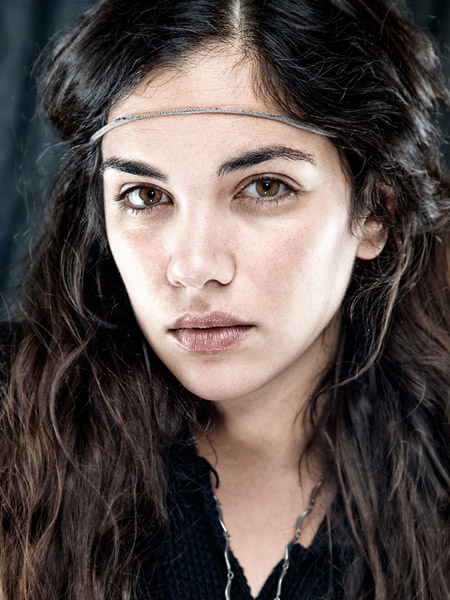
\includegraphics[height=5cm]{./images/amato.jpg}\hfill}
\else
  \hbox to \textwidth{\hfill 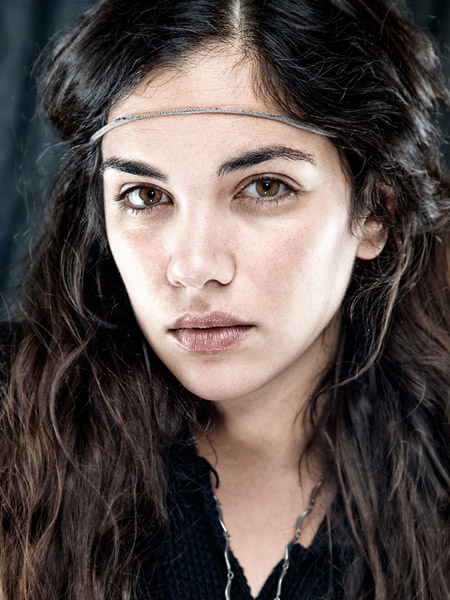
\includegraphics[height=10cm]{./images/amato.jpg}}
\fi
\end{figure}

If we add some code then it will float on the next page, but first let us refresh how we can measure the height and width of the image.
\newbox\imgbox
\begin{scriptexample}{}{}
\begin{verbatim}
\newbox\imgbox
\setbox\imgbox= \hbox{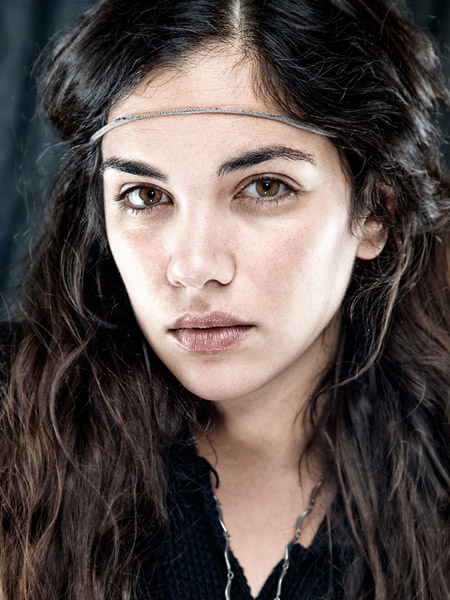
\includegraphics[height=2cm]{./images/amato.jpg}}%

Width of image is \the\wd\imgbox and the height is \the\ht\imgbox
\end{verbatim}
\end{scriptexample}

This will result in:

\begin{scriptexample}{}{}
\setbox\imgbox= \hbox{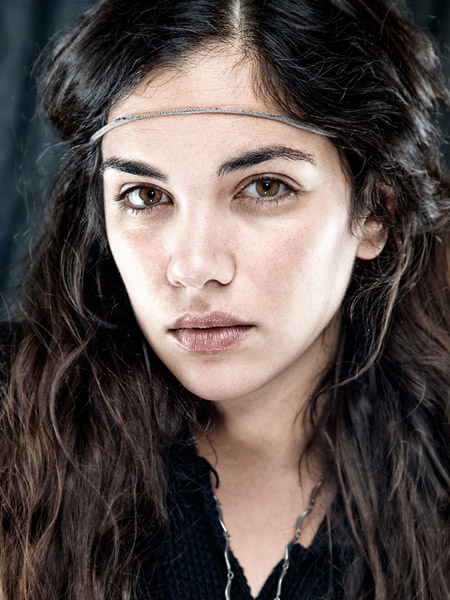
\includegraphics[height=2cm]{./images/amato.jpg}}%
Width of image is \the\wd\imgbox\ and the height is \the\ht\imgbox  
\end{scriptexample}

This simple procedure will be used fairly often, we will place material in a box and then measure its width and height in order to have TeX calculate its dimensions, which can be used later to do more intelligent things with images. 

\begin{figure}[tb]
\ifoddpage
  \hbox to \textwidth{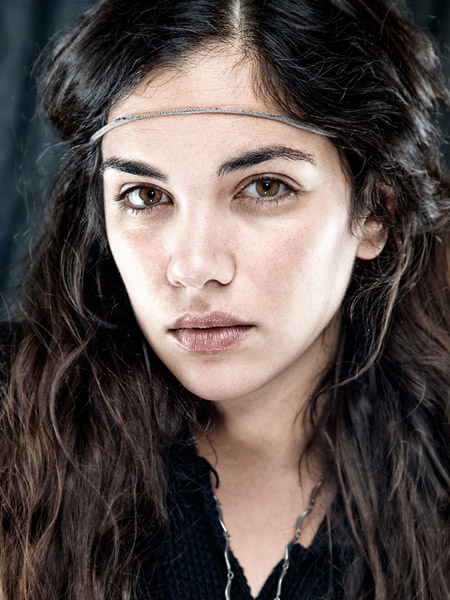
\includegraphics[height=3cm]{./images/amato.jpg}\hfill}%
\else
  \hbox to \textwidth{\hfill 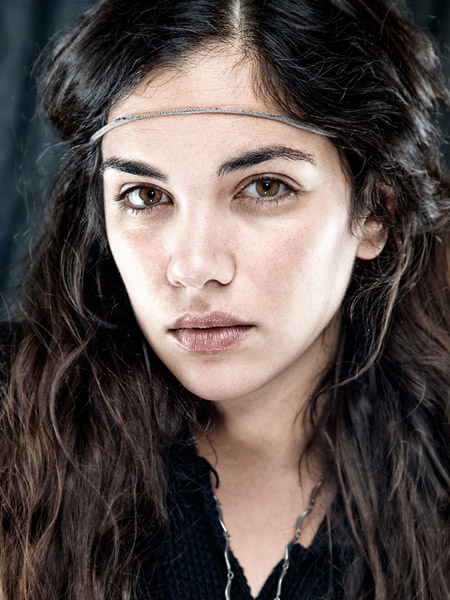
\includegraphics[height=4cm]{./images/amato.jpg}}%
\fi
\end{figure}


\section{Customizing Float Placement}

The automatic placement of figures by \latexe are controlled by a set of counters and macros. These counters do not affect float pages. Specifying [!] in the float placement option causes \latex to ignore these parameters. The values of these counters are set with the \cs{setcounter} command. For example,

\begin{verbatim}
\setcounter{topnumber}{4}
\end{verbatim}

\begin{table}[htbp]
\caption{Float Placement Counters}
\centering
\begin{tabularx}{0.8\textwidth}{|l|X|}
\hline
|topnumber| & The maximum number of floats allowed at the top of a text page (the default is 2).\\
\hline
|bottomnumber| &The maximum number of floats allowed at the bottom of a text
page (the default is 1).\\
\hline
|totalnumber| &The maximum number of floats allowed on any one text page
(the default is 3)\\
\hline
\end{tabularx}
\end{table}

\reversemarginpar

\section{Placement Fraction Guidelines}

\begin{macro}{\textfaction}
    Setting \textfraction smaller than 0.15 is discouraged as it produces hardto-read
    pages. If a figure’s height is more than 85\% of \cmd{\textheight}, it almost
    certainly looks better by itself on a float page than squeezed on a text page
    with a couple of lines of text below it.
    
    Setting \cmd{\textfraction} to zero as permits a text page to have
   no text, which confuses \latex and leads to badly-formatted pages.
\end{macro}
%
\begin{macro}{\topfraction}
Never set \cmd{\topfraction} larger than 1 - \cmd{\textfraction}, as that causes contradictions
in the float-placing algorithm.
\end{macro}

\begin{quote}
\begin{verbatim}
\renewcommand{\topfraction}{.85}
\renewcommand{\bottomfraction}{.7} % .3 in kernel.
\renewcommand{\textfraction}{.15}
\renewcommand{\floatpagefraction}{.7}
\renewcommand{\dbltopfraction}{.66}
\renewcommand{\dblfloatpagefraction}{.66}
\setcounter{topnumber}{9}
\setcounter{bottomnumber}{9}
\setcounter{totalnumber}{20}
\setcounter{dbltopnumber}{9}
\end{verbatim}
\end{quote}

\section{The float package}
 
The \docpkg{float} package provides a friendly interface to define image new float objects. Moreover, the package
defines certain \emph{float styles} that can be used to define new floating objects.  It
was designed by Anselm Lingnau. New float objects can be defined with the command.\index{floats>float styles}

\begin{verbatim}
\newfloat{type}{placement}{ext }[within]
\end{verbatim}



Here type is the \emph{type}  of the new class of floats (e.g., program, diagram, photo, etc.),
placement gives the default placement specifier, and |ext| is the filename extension
for the file that will keep the captions in cases where we want to have a list of programs,
list of diagrams, or other lists. The optional argument within is used to number float
objects within some sectioning unit (e.g.,chapter, section). Here is a complete example:

\begin{teXXX}
\floatstyle{plain}
\newfloat{Photo}{htbp}{fot}[section]
\end{teXXX}




\floatstyle{plain}
\newfloat{Photo}{htbp}{fot}

\begin{Photo}
 \centering
 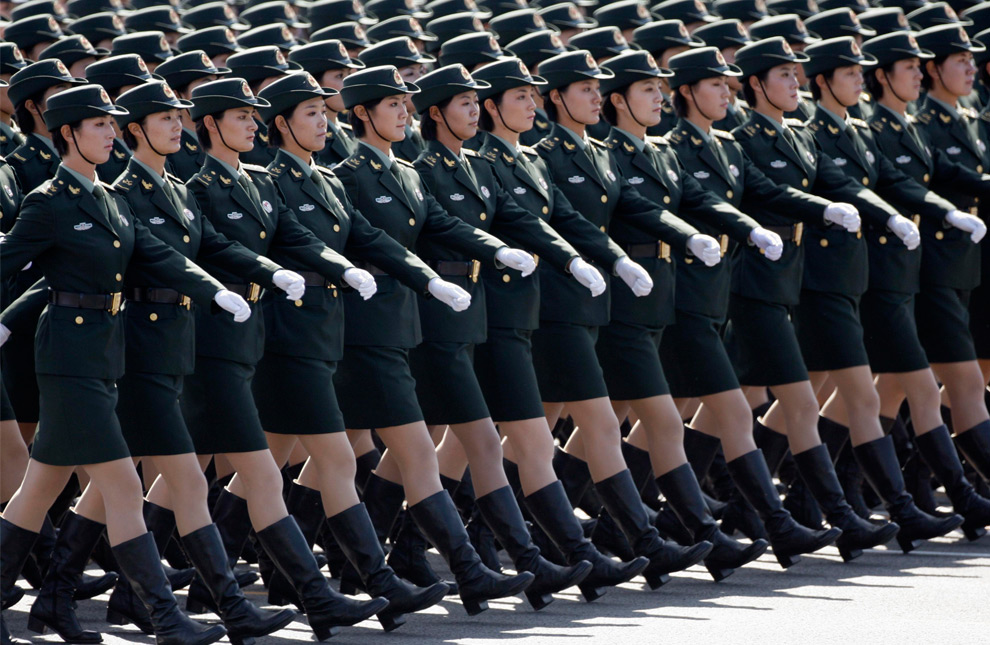
\includegraphics[width=0.80\linewidth]{./images/china-05.jpg}
\caption[a short caption]{If the caption is very long it is formatted as a paragraph, which is flushleft. If it is short it will be centered. }
\end{Photo}


\begin{Photo}
 \centering
 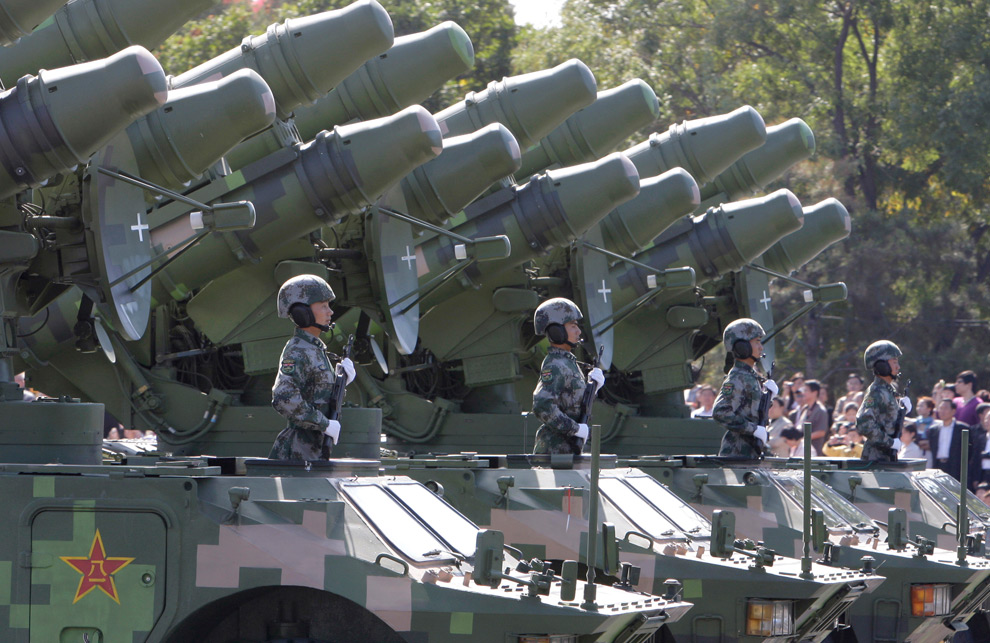
\includegraphics[width=0.80\linewidth]{./images/china-06.jpg}
\caption{. . . caption . . . }
\end{Photo}

\begin{Photo}
 \centering
 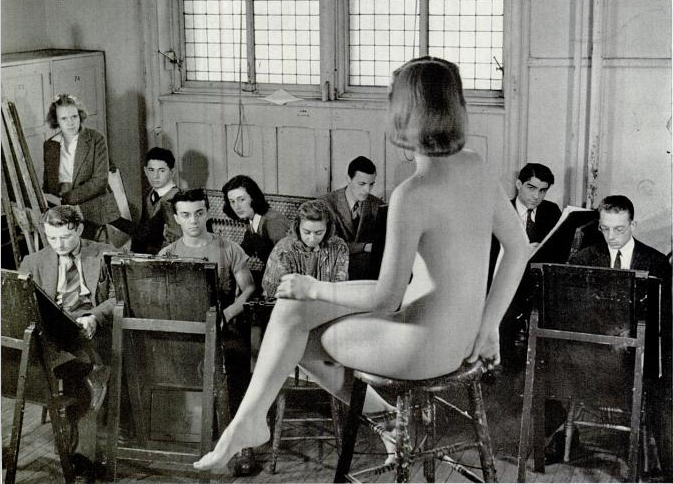
\includegraphics[width=0.65\linewidth]{./images/yaleartschool.png}
\caption{. . . caption . . . }
\end{Photo}



Note that after each such definition, a new 
environment will be available. Naturally,
its name depends on the `type' (e.g., the example code above will create the program
environment). The `float style' can be specified with the \cs{floatstyle} command. The
command takes only one argument, which is the name of a ‘‘float style’’:

\begin{teXXX}
\begin{Example}
     First verbatim line.
     Second verbatim line.
     Third verbatim line.
\end{Example}
\end{teXXX}



\floatstyle{ruled}
\newfloat{Example}{htbp}{loe}[chapter]

 \begin{Example}
 \begin{verbatim}
   \begin{Photo}
      \centering
      \includegraphics[width=0.65\linewidth]{./graphics/level3.jpg}
      \caption{. . . caption . . . }
   \end{Photo}
\end{verbatim}
\caption{Example using verbatim code}
 \end{Example}

\begin{Photo}
 \centering
 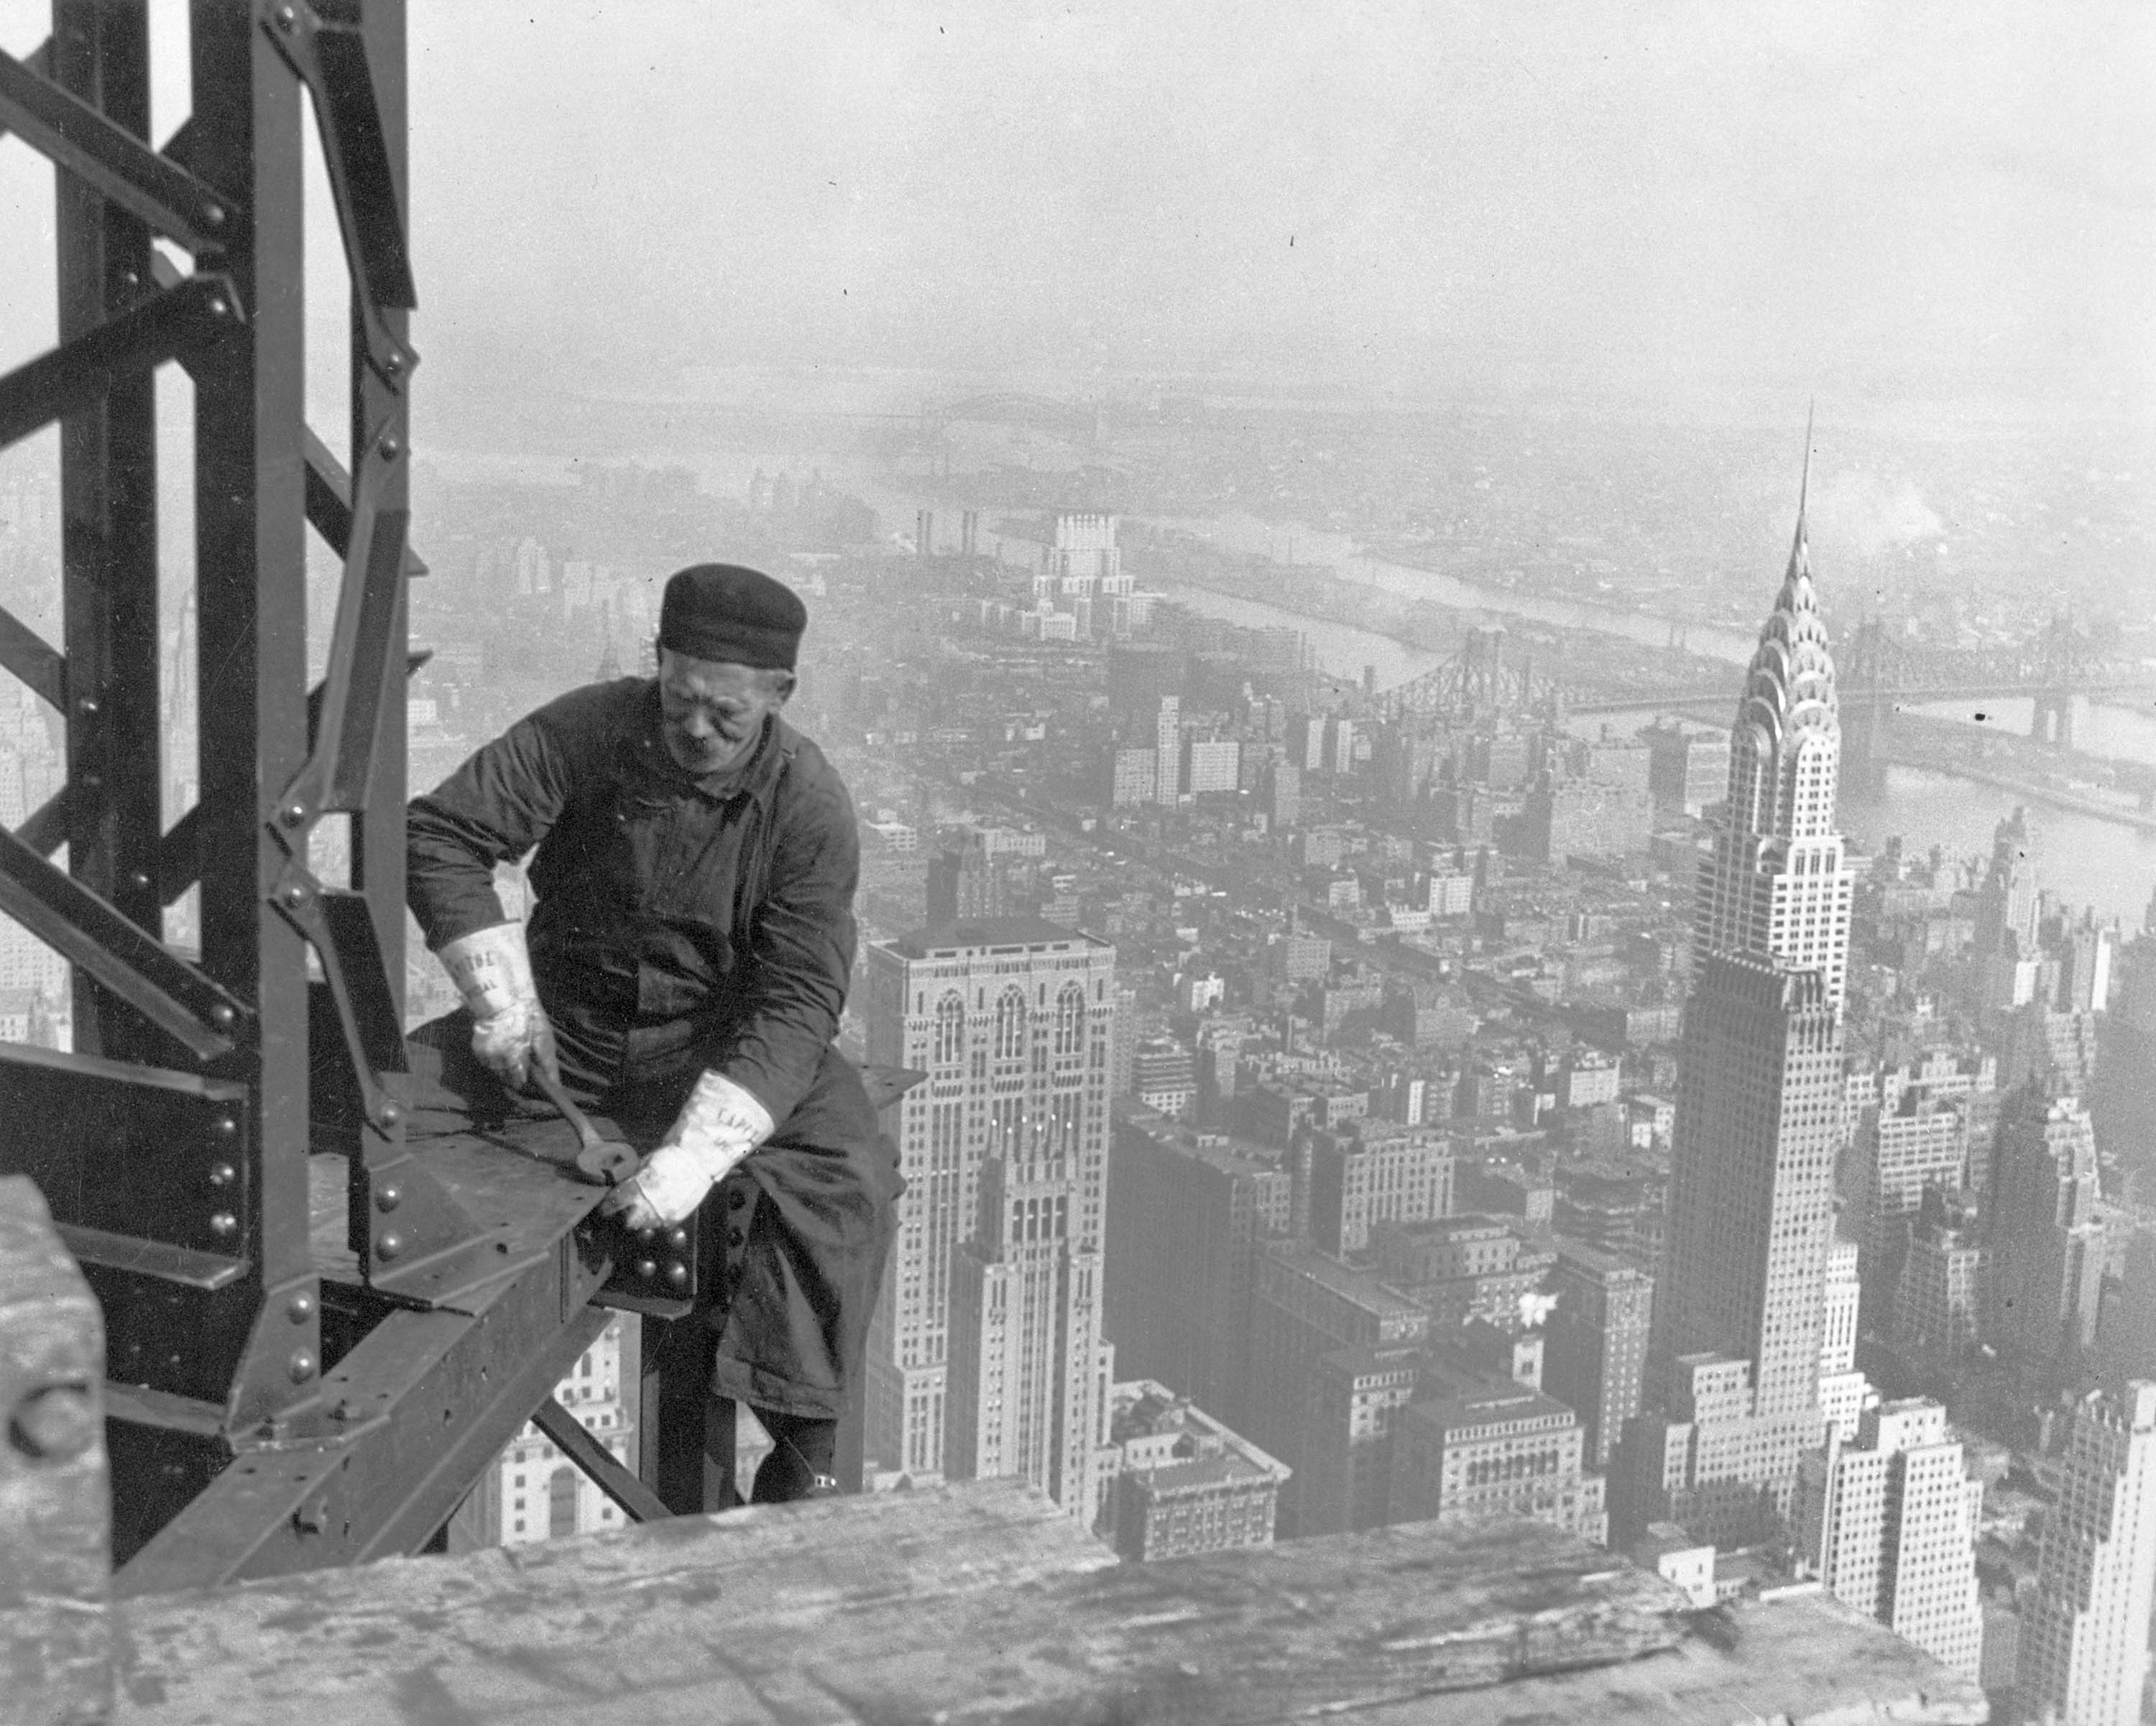
\includegraphics[width=0.85\linewidth]{./images/old-timer-structural-worker.jpg}
\caption{. . . caption . . . }
\end{Photo}


                                             
\begin{plate}[h]
\caption{This is a plate}
 \end{plate}                                             


\begin{painting}[h]
\caption{This is a plate}
 \end{painting} 

